\chapter{Introduction}
\label{chap:introduction}
<INTRODUCTIE TEKST>
\section{Motivation}
% \subsection{Origin and history}
In 2008 Thijs van As designed the first version of the $\rho$-VEX processor \cite{As:2008rt}. This processor uses a VLIW design and is based on the VEX ISA. The VEX ISA is a derivative of the Lx family of embedded VLIW processors \cite{854391} from HP/STMicroelectronics.
Around this processor a set of tools has been developed in collaboration with the TU Delft, IBM, STMicroelectronics and other universities. Currently the $\rho$-VEX 2.0 tool suite include a synthesizable core, a compiler system and a processor simulator. A GCC based VLIW compiler has been developed by IBM.  
A Very Long Instruction Word (VLIW) processor can execute multiple operations during a single clock cycle. A compiler is required to find parallelism between instructions and to provide scheduling that enables the VLIW processor to execute multiple operations during a single cycle.

A regular RISC type processor, such as the MIPS and ARM processor, contain a single instruction pipeline that executes instructions. Figure \ref{fig:mips_pipe} shows a basic MIPS integer pipeline. By introducing pipelining registers the clock frequency of a processor can be increased because execution of an instruction is broken up into smaller and simpler parts. A pipeline can contain multiple instructions that are in different stages of execution.

\begin{figure}[ht]
\centering
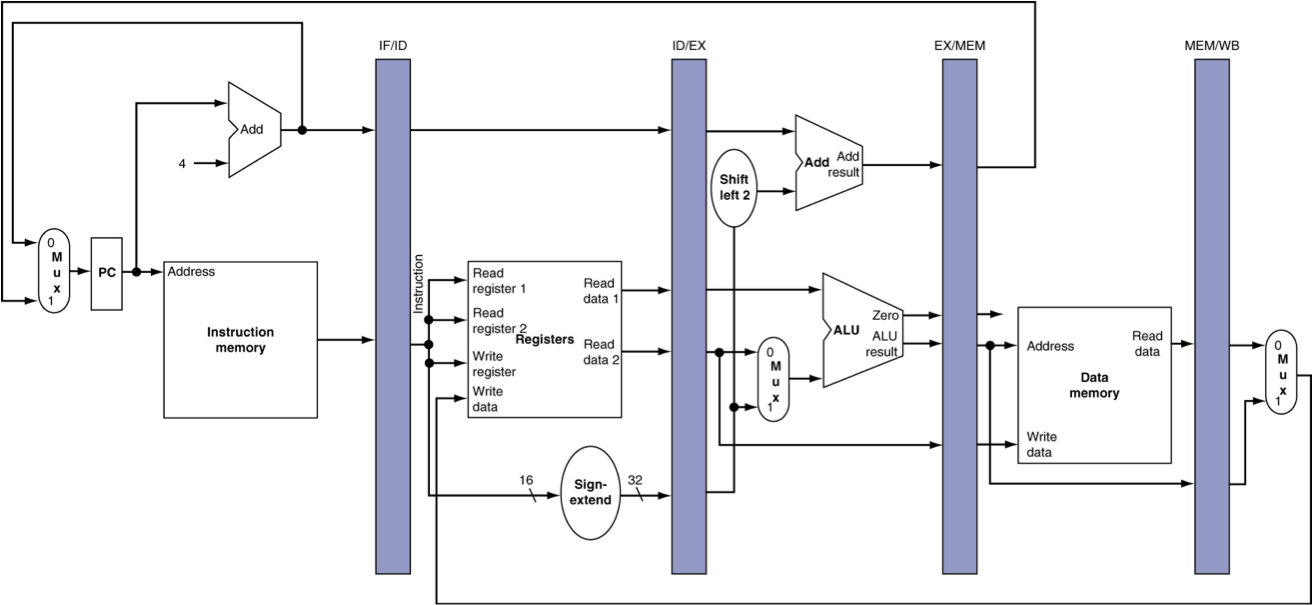
\includegraphics[width=0.8\textwidth]{1_introduction/img/MIPS_pipe.png}
\caption{MIPS pipeline \cite{John-L.-Hennessy:2009wq}}
\label{fig:mips_pipe}
\end{figure}

Introducing pipelining will generally lower the Clocks Per Instruction (CPI) rate of a processor to below 1.0. Special hardware has been developed, such as forwarding units, branch predictors, and speculative execution that will try to increase the CPI to a value that approaches 1.0. 

If a higher then 1.0 CPI is desired multiple instructions need to be executed during a single clock cycle. Machines that can execute multiple instructions are called multi issue machines. These types of processors use special hardware to find dependencies between instructions and to determine which instructions can be executed in parallel. These techniques include Tomasulo’s algorithm for Out of Order execution and register renaming. Most modern processors use these techniques to increase performance.

Finding dependencies between instructions becomes increasingly complex when the issue width of machines is increased. The Pentium 4 processor demonstrated the limitations of further ILP extraction in a spectacular way. It used a 20-stage pipeline \cite{John-L.-Hennessy:2012bs} with seven functional units. It operated on RISC-like micro-ops instead of x86 instructions and could handle 50 in-flight instructions at a time.

The amount of silicon and energy that was dedicated to finding and executing ILP made the Pentium 4 processor very inefficient. The expected clock frequency increase that Intel expected the hyper pipelined processor (6-7 GHz) to deliver never materialized and the Pentium 4 Netburst architecture was dropped for a much simpler architecture.

\cite{Wall:1993xy} showed the actual limitations of ILP extraction in hardware and demonstrated that other techniques need to be used to find and execute more ILP.

VLIW differs from multiple issue machines in that parallelism is found during compile-time instead of during run-time. This results in a processor that can be made significantly simpler because the ILP extraction algorithms do not need to be implemented and because dependency checking is not required during run-time. Additional ILP can also be found with the compiler because the compiler has got a higher level view of the code that is to be executed. Optimizations such as swing modulo scheduling and loop vectorization are nearly impossible to achieve in hardware because the higher level structure is no longer available. A compiler can interpret the higher level structure of a program and optimize the output for better scheduling.

The origins of the VEX ISA can be traced to the company Multiflow and John Fisher, one of the inventors of VLIW processors at Yale University \cite{Fisher:1983:VLI:1067651.801649}. Multiflow designed a computer that used VLIW processors to execute instructions up to 1024-bit in size. Along with these computers Multiflow also designed a compiler system that used trace based scheduling to extract ILP from programs. Reportedly the code base for the Multiflow compiler has been used in modern compiler such as Intel C Compiler (ICC) and HP VEX compiler because of the robustness and the amount of ILP that could be exposed by the compiler \cite{Lowney:1993qy}.

John Fisher has designed the VEX ISA as an example of VLIW type processors \cite{Joseph-A.-Fisher:2005cr}. His work includes the design of a VLIW processor and ISA and a compiler system that generates code for this processor.

Currently two different compilers exist that target the $\rho$-VEX processor: the VEX compiler and a GCC port developed by IBM. We will show that both existing compilers are not optimal and that a new compiler is required for the $\rho$-VEX project. Further we will present a LLVM based compiler that targets the $\rho$-VEX processor with performance and features similar to the VEX compiler. 

\section{Problem statement}
Currently, both the HP-VEX and GCC compilers can be used to generate code for the $\rho$-VEX processor. Both compilers have got a number of advantages and disadvantages that will be explored. The compilers will be judged on the following subjects: Code quality, support, languages support, backend supported and customization possibilities.
\newline

% \begin{itemize}
% 	\item \textbf{Code quality:}
% 	\item \textbf{Support:}
% 	\item \textbf{Front-end:}
% 	\item \textbf{Back-end:}
% 	\item \textbf{Customization:}
% \end{itemize}
HP-VEX:
\begin{itemize}
	\item \textbf{Code quality:} Excellent code quality and ILP extraction.
	\item \textbf{Support:} Bad, no active community.
	\item \textbf{Front-end:} Bad, only support for C.
	\item \textbf{Back-end:} Not applicable since compiler is specifically targeted to one architecture.
	\item \textbf{Customization:} Customization possible through machine description. Further research on optimization strategies not possible because compiler is proprietary and closed source. Because of this expanding the functionality of the compiler is impossible.
\end{itemize}

GCC:
\begin{itemize}
	\item \textbf{Code quality:} Excellent code quality with performance approaching that of commercial compilers (CITATION NEEDED).
	\item \textbf{Support:} There is a very active development community around GCC.
	\item \textbf{Front-end:} GCC supports a large number of programming languages including C, C++, Fortran and Java
	\item \textbf{Back-end:} Supoort exists for a large number of processors including x86, ARM, MIPS and ofcourse VEX
	\item \textbf{Customization:} Because GCC is open source the compiler can be customized to support new passes, optimizations and instructions.
\end{itemize}

Unfortunately GCC has a number of disadvantages that need mentioning.

\begin{itemize}
	\item \textbf{VEX code quality:} The VEX backend for GCC has not been optimized and the quality of the code is quite low. Performance of GCC executables is lower then code compiled by the HP-VEX compiler. Some programs do not function correclty when compiled by GCC. Some programs are unable to be compiled by GCC.
	\item \textbf{VEX reconfiguration:} The current GCC VEX compiler does not support run-time reconfiguration. The compiler has been set to a 4 issue width $\rho$-VEX and this cannot be changed without rebuilding GCC.	
	\item \textbf{Bloated:} GCC consists of millions of lines of code and is arguable one of the most complex programs in existence. This makes understanding GCC and developing for GCC very hard.
	\item \textbf{Complexity:} GCC is written in C. Design is complex, not very modular and documentation is not very good. Different parts of the compiler are linked in a complex way and it is very difficult to obtain a general picture on how the compiler operates. Because of the complexity it is difficult to achieve high performance in GCC.
\end{itemize}

The comparison shows that both the HP-VEX and GCC compilers have serious disadvantages. The fact that HP-VEX cannot be customized excludes it from further development for the $\rho$-VEX project. Bringing the GCC compiler performance and features up to the same level as HP-VEX will be very difficult because of the complexity involved with GCC development.  

In 2000 the LLVM project has been started with the goal of replacing the code generator in the GCC compiler. LLVM provides a modern, modular design and is written in C++. The GCC front-end was used to translate programs into LLVM compatibale intermediate representation. Around 2005 the Clang project was started which aimed to replace the GCC front-end with an independent front-end with support for C, C++ and ObjC. Currently the LLVM based compiler offers performance that approaches GCC but offering a significant improvement in terms of modularity, ease of development and "hackability". In addition the LLVM compiler can also be used to target different architectures such as GPU's and VLIW based processors.

\subsection{Goals}
The main goal of this thesis is to develop a new compiler for the $\rho$-VEX system. The compiler will be based on the LLVM compiler. The new compiler should have the following characteristics:

\begin{itemize}
	\item \textbf{Open source:} The compiler should be open source so the compiler can be customized and used for future research.
	\item \textbf{Code quality:} A new compiler should provide a significant improvement in terms of performance, code size and resource utilization.
	\item \textbf{Reconfigurability:} Charachteristics of the $\rho$-VEX processor should be reconfigurable during run-time.
\end{itemize}

\section{Methodology}
The following steps need to be completed for successful implementation of a $\rho$-VEX LLVM compiler.
\begin{itemize}
	\item Research $\rho$-VEX and VEX platform
	\item Research LLVM compiler framework
	\item Build LLVM based VEX compiler with following features:
	\begin{itemize}
		\item 4 issue width VLIW
		\item Code generation
		\item Assembly emitter
	\end{itemize}
	\item Add support for reconfigurability
		\begin{itemize}
			\item VEX machine description
			\item Reconfigure LLVM during runtime
		\end{itemize}	
	\item Optimize performance
	\begin{itemize}
		\item Instruction selection
		\item Hazard recognizer
		\item Register allocator
	\end{itemize}	
\end{itemize}




\section{Thesis overview}
The thesis is organized as follows. 
In Chapter \ref{chap:background} we will discuss the architecture of the $\rho$-VEX processor and the workings of the LLVM compiler suite. This chapter will demonstrate the supported instructions, run-time architecture, and show the general architecture of the $\rho$-VEX processor. The chapter will also show how the LLVM compiler operates and what steps are involved during compilation.

In Chapter \ref{chap:implementation} will discuss how the $\rho$-VEX compiler was implemented.  This chapter will present how a back-end is implemented in LLVM. We will show how code is transformed from the LLVM Intermediate Representation into a $\rho$-VEX specific assembly language. In addition we will also discuss new functionality that has been added to the LLVM compiler.

Chapter \ref{chap:optimization} will discuss how the performance of the LLVM compiler has been optimized. Problems that have been found are demonstrated and we will show how these problems have been solved to increase performance of the binaries.

Chapter \ref{chap:results} will explore the performance of the new compiler. Performance will be compared to existing compilers in terms of issue width, optimization levels and other metrics. A conclusion and recommendations for future research is presented in chapter \ref{chap:conclusion}.  


\acresetall
